%-*- coding:utf-8 -*-

\documentclass[10pt,dvipdfmx]{beamer}
\usepackage{tutorial}

\title{計算機実験II (L8) --- 最適化(2)}
\date{2020/12/11}

\begin{document}

\begin{frame}
  \titlepage
  \tableofcontents
\end{frame}

\begin{frame}[t]{講義日程}
  \begin{itemize}
    % \setlength{\itemsep}{1em}
  \item 全8回 (金曜5限 {\color{red}17:05}-18:35)
    \begin{itemize}
    \item {\color{gray} 10月8日 第1回: 乱択アルゴリズム、モンテカルロ法}
    \item 10月15日 第2回: 多体系の統計力学、マルコフ連鎖モンテカルロ法
    \item 10月22日 第3回
    \item 10月29日 第4回
    \item 11月5日 休講 (もくもく会)
    \item 11月12日 休講 (物理学教室コロキウム)
    \item 11月19日 第5回
    \item 11月26日 休講 (物理学教室コロキウム)
    \item 12月3日 第6回
    \item 12月10日 第7回
    \item 12月17日 休講 (物理学教室コロキウム)
    \item 12月24日 第8回
    \item 1月7日 休講 (もくもく会)
    \item 1月18日(火) 休講 (予備日)
    \end{itemize}
  \end{itemize}
\end{frame}


\section{最適化問題}

\begin{frame}[t,fragile]{最適化問題}
  \begin{itemize}
    %\setlength{\itemsep}{1em}
  \item 目的関数(コスト関数)$f(x)$の最小値(あるいは最大値)とその場所を求めたい
  \item どういう問題を解くのに使えるか?
    \begin{itemize}
    \item 変分原理が成り立つ問題: 最小作用の原理、最小エネルギーの原理$\cdots$
    \item 目的関数が定義できる問題: 最小二乗法(線形回帰、非線形回帰)、(連立)方程式、常/偏微分方程式、機械学習$\cdots$
    \end{itemize}
  \item ほぼ全ての問題は、目的関数をうまく定義することで最適化問題に書き換えることができる
    \begin{itemize}
    \item (一般に)最適化問題として解くのは最終手段
    \item それぞれの問題に特化したより良い方法があるときはそちらを使う
    \end{itemize}
  \end{itemize}
\end{frame}

\begin{frame}[t,fragile]{様々な最適化手法}
  \begin{itemize}
    %\setlength{\itemsep}{1em}
  \item 最適化問題の種類
    \begin{itemize}
    \item 連続最適化問題 $\Leftarrow$ 目的関数が凸ではない場合、難しい
    \item 離散最適化(組み合せ最適化)問題 $\Leftarrow$ さらに難しい
    \end{itemize}
  \item 真の(大局的な)最小値(最大値)を求めるのは難しい
  \item 一般的には極値を求めることしかできない
  \item 多次元では極小を囲い込むことができない
  \item 導関数を使う方法: ニュートン法、準ニュートン法、最急降下法、勾配降下法、共役勾配法$\cdots$
  \item 使わない方法: 囲い込み法、Nelder-Meadの滑降シンプレックス法、シミュレーテッドアニーリング、量子アニーリング$\cdots$
  \item 目的関数・導関数の評価回数と収束までの反復回数のトレードオフ
  \end{itemize}
\end{frame}


\section{Nelder-Meadの滑降シンプレックス法}

\begin{frame}[t,fragile]{Nelder-Meadの滑降シンプレックス法}
  \begin{itemize}
    %\setlength{\itemsep}{1em}
  \item 関数値のみ。導関数の情報を必要としない
  \item プログラミングが簡単
  \item 収束は遅いが、安定に極小値が求まる
  \item $d+1$個の頂点からなる$d$次元の超多面体(シンプレックス)を変形しながら、極小値を探す
    \begin{itemize}
    \item 2次元: 三角形
    \item 3次元: 四面体
    \end{itemize}
  \item 別名「アメーバ法」
  \end{itemize}
\end{frame}

\begin{frame}[t,fragile]{Nelder-Meadの滑降シンプレックス法}
  \begin{itemize}
    %\setlength{\itemsep}{1em}
  \item $d+1$個の点$x_0,x_1,\cdots,x_d$は$f(x_0) \le f(x_1) \le \cdots \le f(x_d)$の順に並べられているとする
  \item 最大値を取る点$x_d$を除く$d$点の重心を$x_g$とする
  \item Nelder-Mead法では以下のステップを繰り返す
    \begin{itemize}
    \item $x_d$を$x_g$に関する対称な点$x_r$に移動(反射)
      \[
      x_r = x_g + (x_g - x_d)
      \]
    \item $f(x_r)$が$f(x_0)$よりも小さい場合、さらに先に進む(拡大)
      \[
      x_e = x_g + 2(x_r - x_g)
      \]
    \item $f(x_r)$が$f(x_{d-1})$よりもまだ大きい場合には、$x_d$を$x_g$に近づける(縮小)
      \[
      x_c = x_g + (x_d-x_g)/2
      \]
    \item $f(x_c)$が$f(x_d)$よりまだ大きい場合には、$x_0$以外の点を$x_0$に一様に近づける(収縮)
      \[
      x_i \leftarrow x_0 + (x_i-x_0)/2 \qquad (i=1 \cdots d)
      \]
    \end{itemize}
  \end{itemize}
\end{frame}


\section{量子アニーリング (復習)}

\begin{frame}[t,fragile]{量子アニーリング}
  \begin{itemize}
    %\setlength{\itemsep}{1em}
  \item 離散最適化問題
    \[
    H = -J \sum_{i<j} \epsilon_{ij} \sigma_i^z \sigma_j^z
    \]
    の基底状態配位と基底状態エネルギーを求めたい
    \begin{center}
      \resizebox{0.6\textwidth}{!}{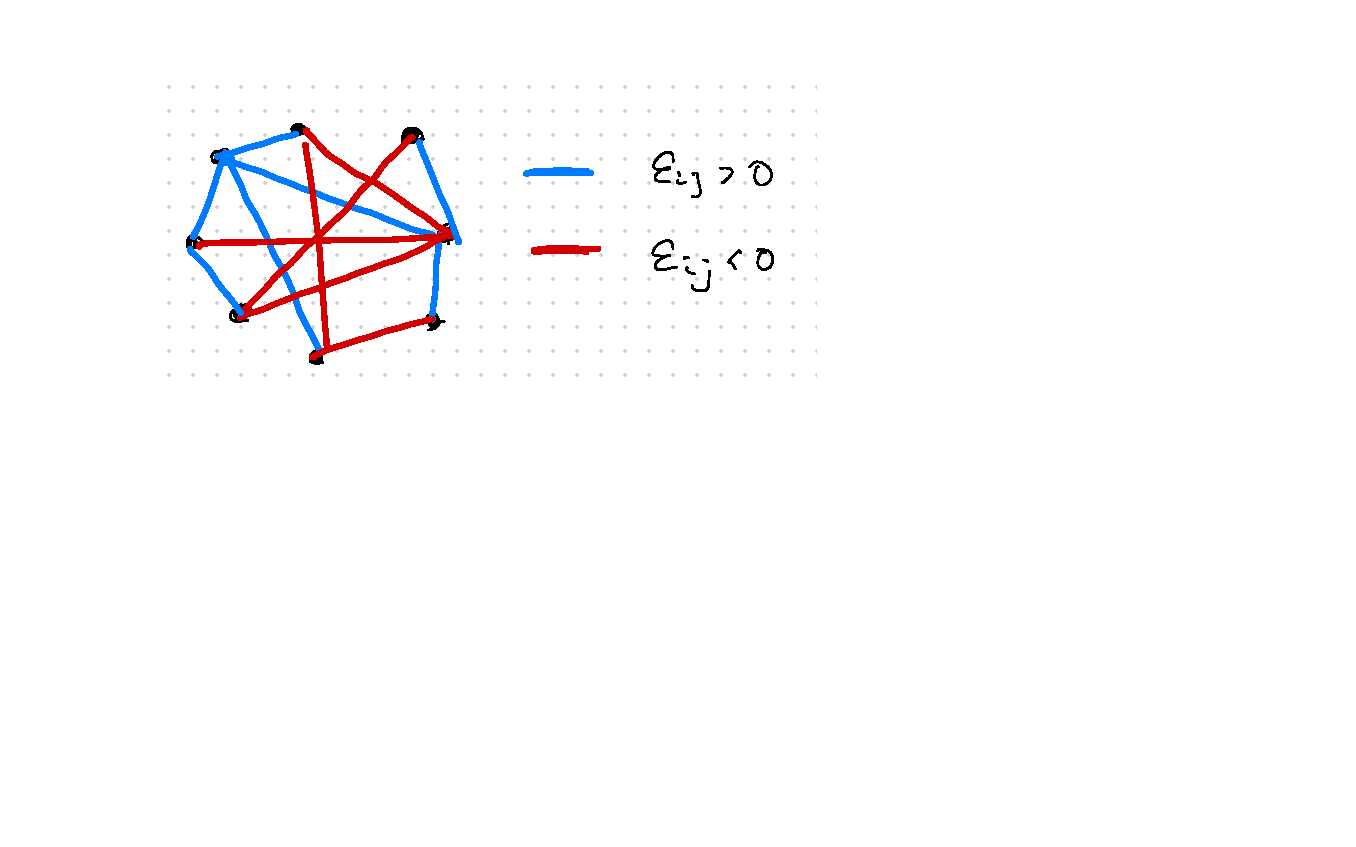
\includegraphics{image/spinglass.pdf}}
    \end{center}
  \end{itemize}
\end{frame}

\begin{frame}[t,fragile]{量子アニーリング}
  \begin{itemize}
    %\setlength{\itemsep}{1em}
  \item 横磁場を導入
    \[
    H = -J \sum_{i<j} \epsilon_{ij} \sigma_i^z \sigma_j^z - \Gamma \sum_i \sigma_i^x
    \]
  \item 古典極限 ($J=1$, $\Gamma=0$)
    \begin{itemize}
    \item 求めたい基底状態
    \end{itemize}
  \item 量子極限 ($J=0$, $\Gamma=1$)
    \begin{itemize}
    \item $2^N$個の全ての状態の重ね合わせ
    \end{itemize}
  \item 量子アニーリング
    \begin{itemize}
    \item $J+\Gamma=1$を保ったままで、$\Gamma=1$から$\Gamma=0$まで「ゆっくり」と減少させながら時間発展させる
      \[
      J = 1-\Gamma = t/T \qquad (0 \le t \le T)
      \]
    \item $T \rightarrow \infty$の極限で確率1で基底状態に収束
    \end{itemize}
  \end{itemize}
\end{frame}


\section{シミュレーテッドアニーリング}

\begin{frame}[t,fragile]{確率過程を用いた最適化}
  \begin{itemize}
    %\setlength{\itemsep}{1em}
  \item 最急降下法 (steepest decent)% {\footnotesize \href{https://github.com/todo-group/computer-experiments/blob/master/exercise/optimization/mc_steepest_descent_1d.c}{mc\_steepest\_descent\_1d.c}}
    \begin{itemize}
    \item 初期状態をランダムに定める
    \item 配位を少しだけ変化させる
    \item エネルギー(コスト関数)が小さくなるなら採択、大きくなるなら棄却 $\Rightarrow$ 絶対零度でのMetropolis法と等価
    \item 状態が変化しなくなるまでくり返す
    \item 問題点 : エネルギー極小状態にすぐに捕まってしまう
    \end{itemize}
  \item 徐冷法 (simulated annealing)% {\footnotesize \href{https://github.com/todo-group/computer-experiments/blob/master/exercise/optimization/simulated_annealing_1d.c}{simulated\_annealing\_1d.c}}
    \begin{itemize}
    \item いきなり温度を零にするのではなく少しずつ下げていく
    \item どれくらいゆっくり下げれば良いか?
      \[
      T(t) \ge cN / \log(t+2)
      \]
    \item 実際には適当なスケジューリングで温度を下げ、何回か繰り返して最も良い結果を採択
    \end{itemize}
  \end{itemize}
\end{frame}

%-*- coding:utf-8 -*-

\begin{frame}[t,fragile]{Metropolis法}
  \begin{itemize}
    %\setlength{\itemsep}{1em}
  \item 現在の配位$x$から、試行配位(trial configuration) $x'$を$x - \Delta \sim x + \Delta$の一様分布より選ぶ
  \item 確率$\min \Big( 1, \frac{e^{-\beta V(x')}}{e^{-\beta V(x)}} \Big)$で$x'$を採択(accept)。棄却(reject)された場合にはもとの$x$のまま
  \item 物理量の測定 (reject された場合にもカウントする)
  \item 採択確率(acceptance probability)は、$\frac{e^{-\beta V(x')}}{e^{-\beta V(x)}+e^{-\beta V(x')}}$でもよい
  \item 例: \href{https://github.com/todo-group/computer-experiments/blob/master/exercise/monte_carlo/harmonic.c}{harmonic.c}
  \end{itemize}
\end{frame}

% -*- coding: utf-8 -*-

\begin{frame}[t,fragile]{最急降下法とシミュレーテッドアニーリング}
  \noindent\resizebox{0.45\textwidth}{!}{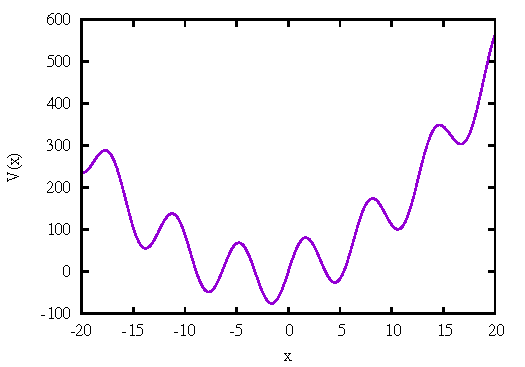
\includegraphics{image/potential.pdf}}

  \noindent\hspace*{.5em}\resizebox{0.43\textwidth}{!}{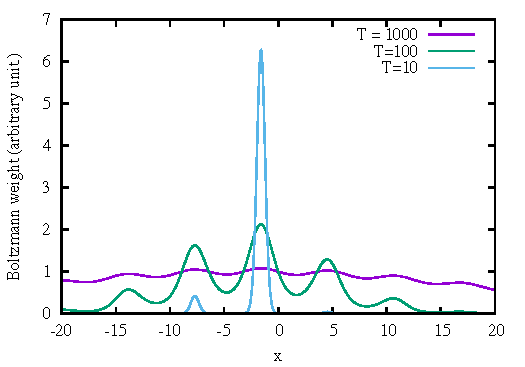
\includegraphics{image/boltzmann.pdf}}

  \vspace*{-17em}\hspace*{12.5em}\resizebox{0.6\textwidth}{!}{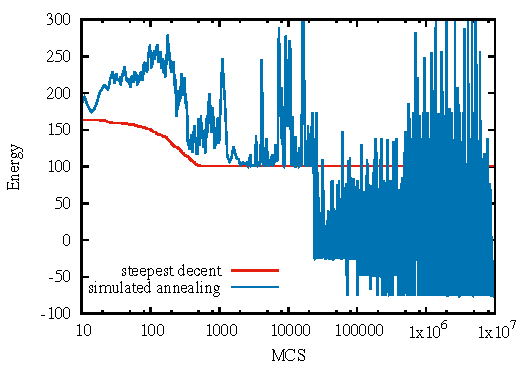
\includegraphics{image/energy.pdf}}

  \hspace*{17em}$T(t) = 100 - \frac{99}{10^7} t$
\end{frame}


\section{最適化手法の比較}

\begin{frame}[t,fragile]{例題 (二次元の最適化)}
  \begin{center}
    \resizebox{.9\textwidth}{!}{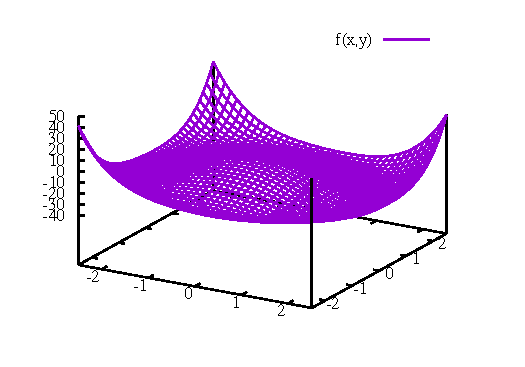
\includegraphics{image/func_2d.pdf}}
  \end{center}
\end{frame}

\begin{frame}[t,fragile]{様々な最適化手法の比較 (1/4)}
  \begin{center}
    \resizebox{.9\textwidth}{!}{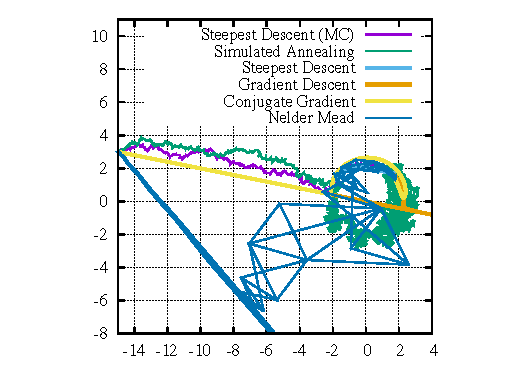
\includegraphics{image/optimization.pdf}}
  \end{center}
\end{frame}

\begin{frame}[t,fragile]{様々な最適化手法の比較 (2/4)}
  \begin{center}
    \resizebox{.9\textwidth}{!}{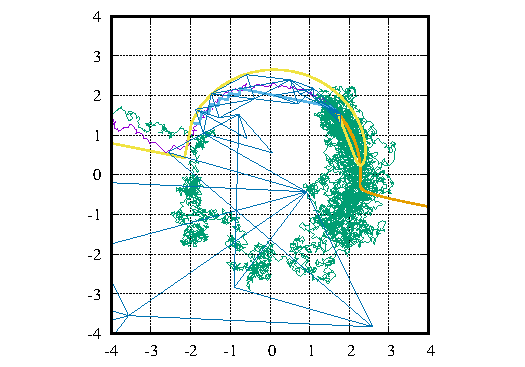
\includegraphics{image/optimization2.pdf}}
  \end{center}
\end{frame}

\begin{frame}[t,fragile]{様々な最適化手法の比較 (3/4)}
  \begin{center}
    \resizebox{.9\textwidth}{!}{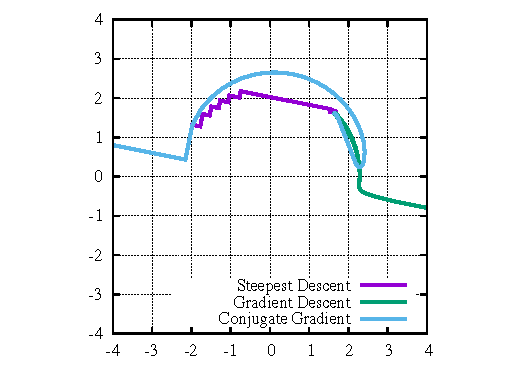
\includegraphics{image/optimization3.pdf}}
  \end{center}
\end{frame}

\begin{frame}[t,fragile]{様々な最適化手法の比較 (4/4)}
  \begin{center}
    \resizebox{.9\textwidth}{!}{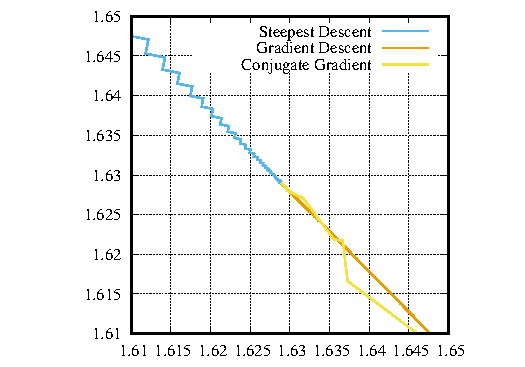
\includegraphics{image/optimization4.pdf}}
  \end{center}
\end{frame}

\begin{frame}[t,fragile]{真の解への近づき方}
  \begin{center}
    \resizebox{.9\textwidth}{!}{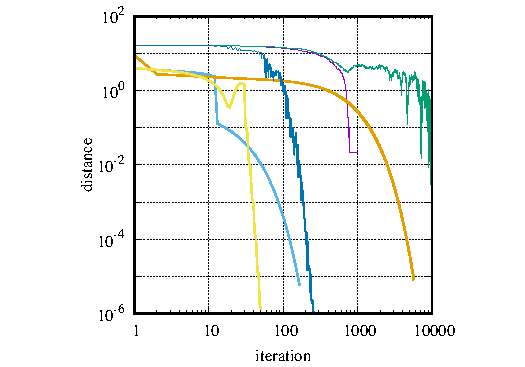
\includegraphics{image/convergence.pdf}}
  \end{center}
\end{frame}


\section{}

\begin{frame}[t,fragile]{計算機環境}
  \begin{itemize}
    %\setlength{\itemsep}{1em}
  \item 教育用計算機システム
  \item 知の物理学クラスタ(ai)
    \begin{itemize}
    \item 卒業まで利用可 (希望すれば大学院でも)
    \item バッチシステムを使えば、かなり大規模な計算も可能
    \end{itemize}
  \item 計算機利用・シミュレーションに関する質問は今後も歓迎 {\tt computer@phys.s.u-tokyo.ac.jp}
  \end{itemize}
\end{frame}

\begin{frame}[t]{本日の課題}
  \begin{itemize}
    %\setlength{\itemsep}{1em}
  \item 実習
    \begin{itemize}
    \item 実習課題一覧\href{https://github.com/todo-group/ComputerExperiments/releases/tag/2020a-computer2}{exercise-2.pdf}から最適化(あるいは別の)課題を選び実習
    \end{itemize}
  \item 質問はSlackの「\# 8\_最適化」あるいは他の適当と思われるチャンネルで
  \item 今回は「作業レポート」はなし
  \item 「レポートNo.2」 (ITC-LMSを参照) 締切 2020/12/25(金)
  \end{itemize}
\end{frame}

\end{document}
